\documentclass{beamer}

\usepackage{pgfpages}
\setbeameroption{show notes on second screen}

\usetheme{CambridgeUS}
\usecolortheme{dolphin}
\usefonttheme{serif}

\definecolor{rit@orange}{HTML}{F36E21}
\definecolor{rit@brown}{HTML}{513127}
\setbeamercolor{structure}{fg=rit@orange}
\setbeamercolor{palette primary}{fg=white, bg=rit@brown}
\setbeamercolor{palette secondary}{fg=rit@brown}
\setbeamercolor{palette tertiary}{fg=white, bg=rit@orange}
\setbeamercolor{titlelike}{fg=rit@brown}
\setbeamercolor{normal text}{fg=rit@brown}

\setbeamertemplate{enumerate}[circle]
\setbeamertemplate{items}[circle]

\AtBeginSection{\frame{\sectionpage}}

\setbeamertemplate{section page}
{
    \begin{centering}
    \begin{beamercolorbox}[sep=12pt,center]{part title}
    \usebeamerfont{section title}\insertsection\par
    \end{beamercolorbox}
    \end{centering}
}

% remove shadow behind blocks
\setbeamertemplate{blocks}[rounded][shadow=false]
% set blocks to use custom color scheme
\setbeamercolor{block title}{bg=rit@orange,fg=white}
\setbeamercolor{block body}{bg=black!5,fg=rit@brown}
% remove shading between block title and body
\makeatletter
\pgfdeclareverticalshading[lower.bg,upper.bg]{bmb@transition}{200cm}{%
  color(0pt)=(lower.bg); color(4pt)=(lower.bg); color(4pt)=(upper.bg)}
\makeatother

\setbeamercovered{dynamic}

\beamertemplatenavigationsymbolsempty

\logo{\vspace{-0.25cm}\includegraphics[width=0.25in]{img/astlogo}}

\pdfpageattr {/Group << /S /Transparency /I true /CS /DeviceRGB>>}

\usepackage{amsmath,amssymb,commath,physics,siunitx,tensor}
\usepackage{aas_macros}
\usepackage{cclicenses,copyrightbox}
\usepackage{float,subcaption}


\usepackage[style=trad-plain,citestyle=authoryear,maxcitenames=3]{biblatex}
\addbibresource{bibliography.bib}


\DeclareCiteCommand{\citefirst}
  {\usebibmacro{prenote}}
  {\renewbibmacro*{name:andothers}{}%
   \usebibmacro{citeindex}%
   \usebibmacro{cite}}
  {\multicitedelim}
  {\usebibmacro{postnote}}

\let\svthefootnote\thefootnote
\textheight 1in
\newcommand\blankfootnote[1]{%
  \let\thefootnote\relax\footnotetext{#1}%
  \let\thefootnote\svthefootnote%
}



\title[Spherical stars]{
  Spherical solutions for stars
}

\author{Daniel Wysocki}

\institute[RIT]{
  Rochester Institute of Technology
}


\date[December 14th, 2015]{
  General Relativity I Presentations
  \\
  December 14th, 2015
}

\begin{document}

\maketitle

\section{Introduction}


\section{Spherically symmetric coordinates}


\begin{frame}{Two-sphere in flat spacetime}

\begin{block}<+->{General metric}
  \begin{displaymath}
    \dd{s}^2 =
   -\dd{t}^2 +
    \dd{r}^2 +
    r^2 (\dd\theta^2 + \sin^2\theta \dd\phi^2)
  \end{displaymath}
\end{block}

\begin{block}<+->{Metric on 2-sphere}
  \begin{displaymath}
    \dd{l}^2 =
    r^2 (\dd\theta^2 + \sin^2\theta \dd\phi^2) \equiv
    r^2 \dd\Omega^2
  \end{displaymath}
\end{block}


\blankfootnote{\textcite[p. 256]{Schutz}}

\end{frame}

%%%%

\begin{frame}{Two-sphere in curved spacetime}

\begin{block}<+->{Metric on 2-sphere}
  \begin{displaymath}
    \dd{l}^2 =
    f(r', t) \dd\Omega^2
  \end{displaymath}
\end{block}

\begin{block}<+->{Relation to $r$}
  \begin{displaymath}
    f(r', t) \equiv r^2
  \end{displaymath}
\end{block}


\blankfootnote{\textcite[pp. 256--257]{Schutz}}

\end{frame}

%%%%

\begin{frame}{Meaning of $r$}

\begin{columns}[c]
  \begin{column}{0.3\textwidth}
    \begin{figure}[ht]
      \centering
      \copyrightbox[r]{
        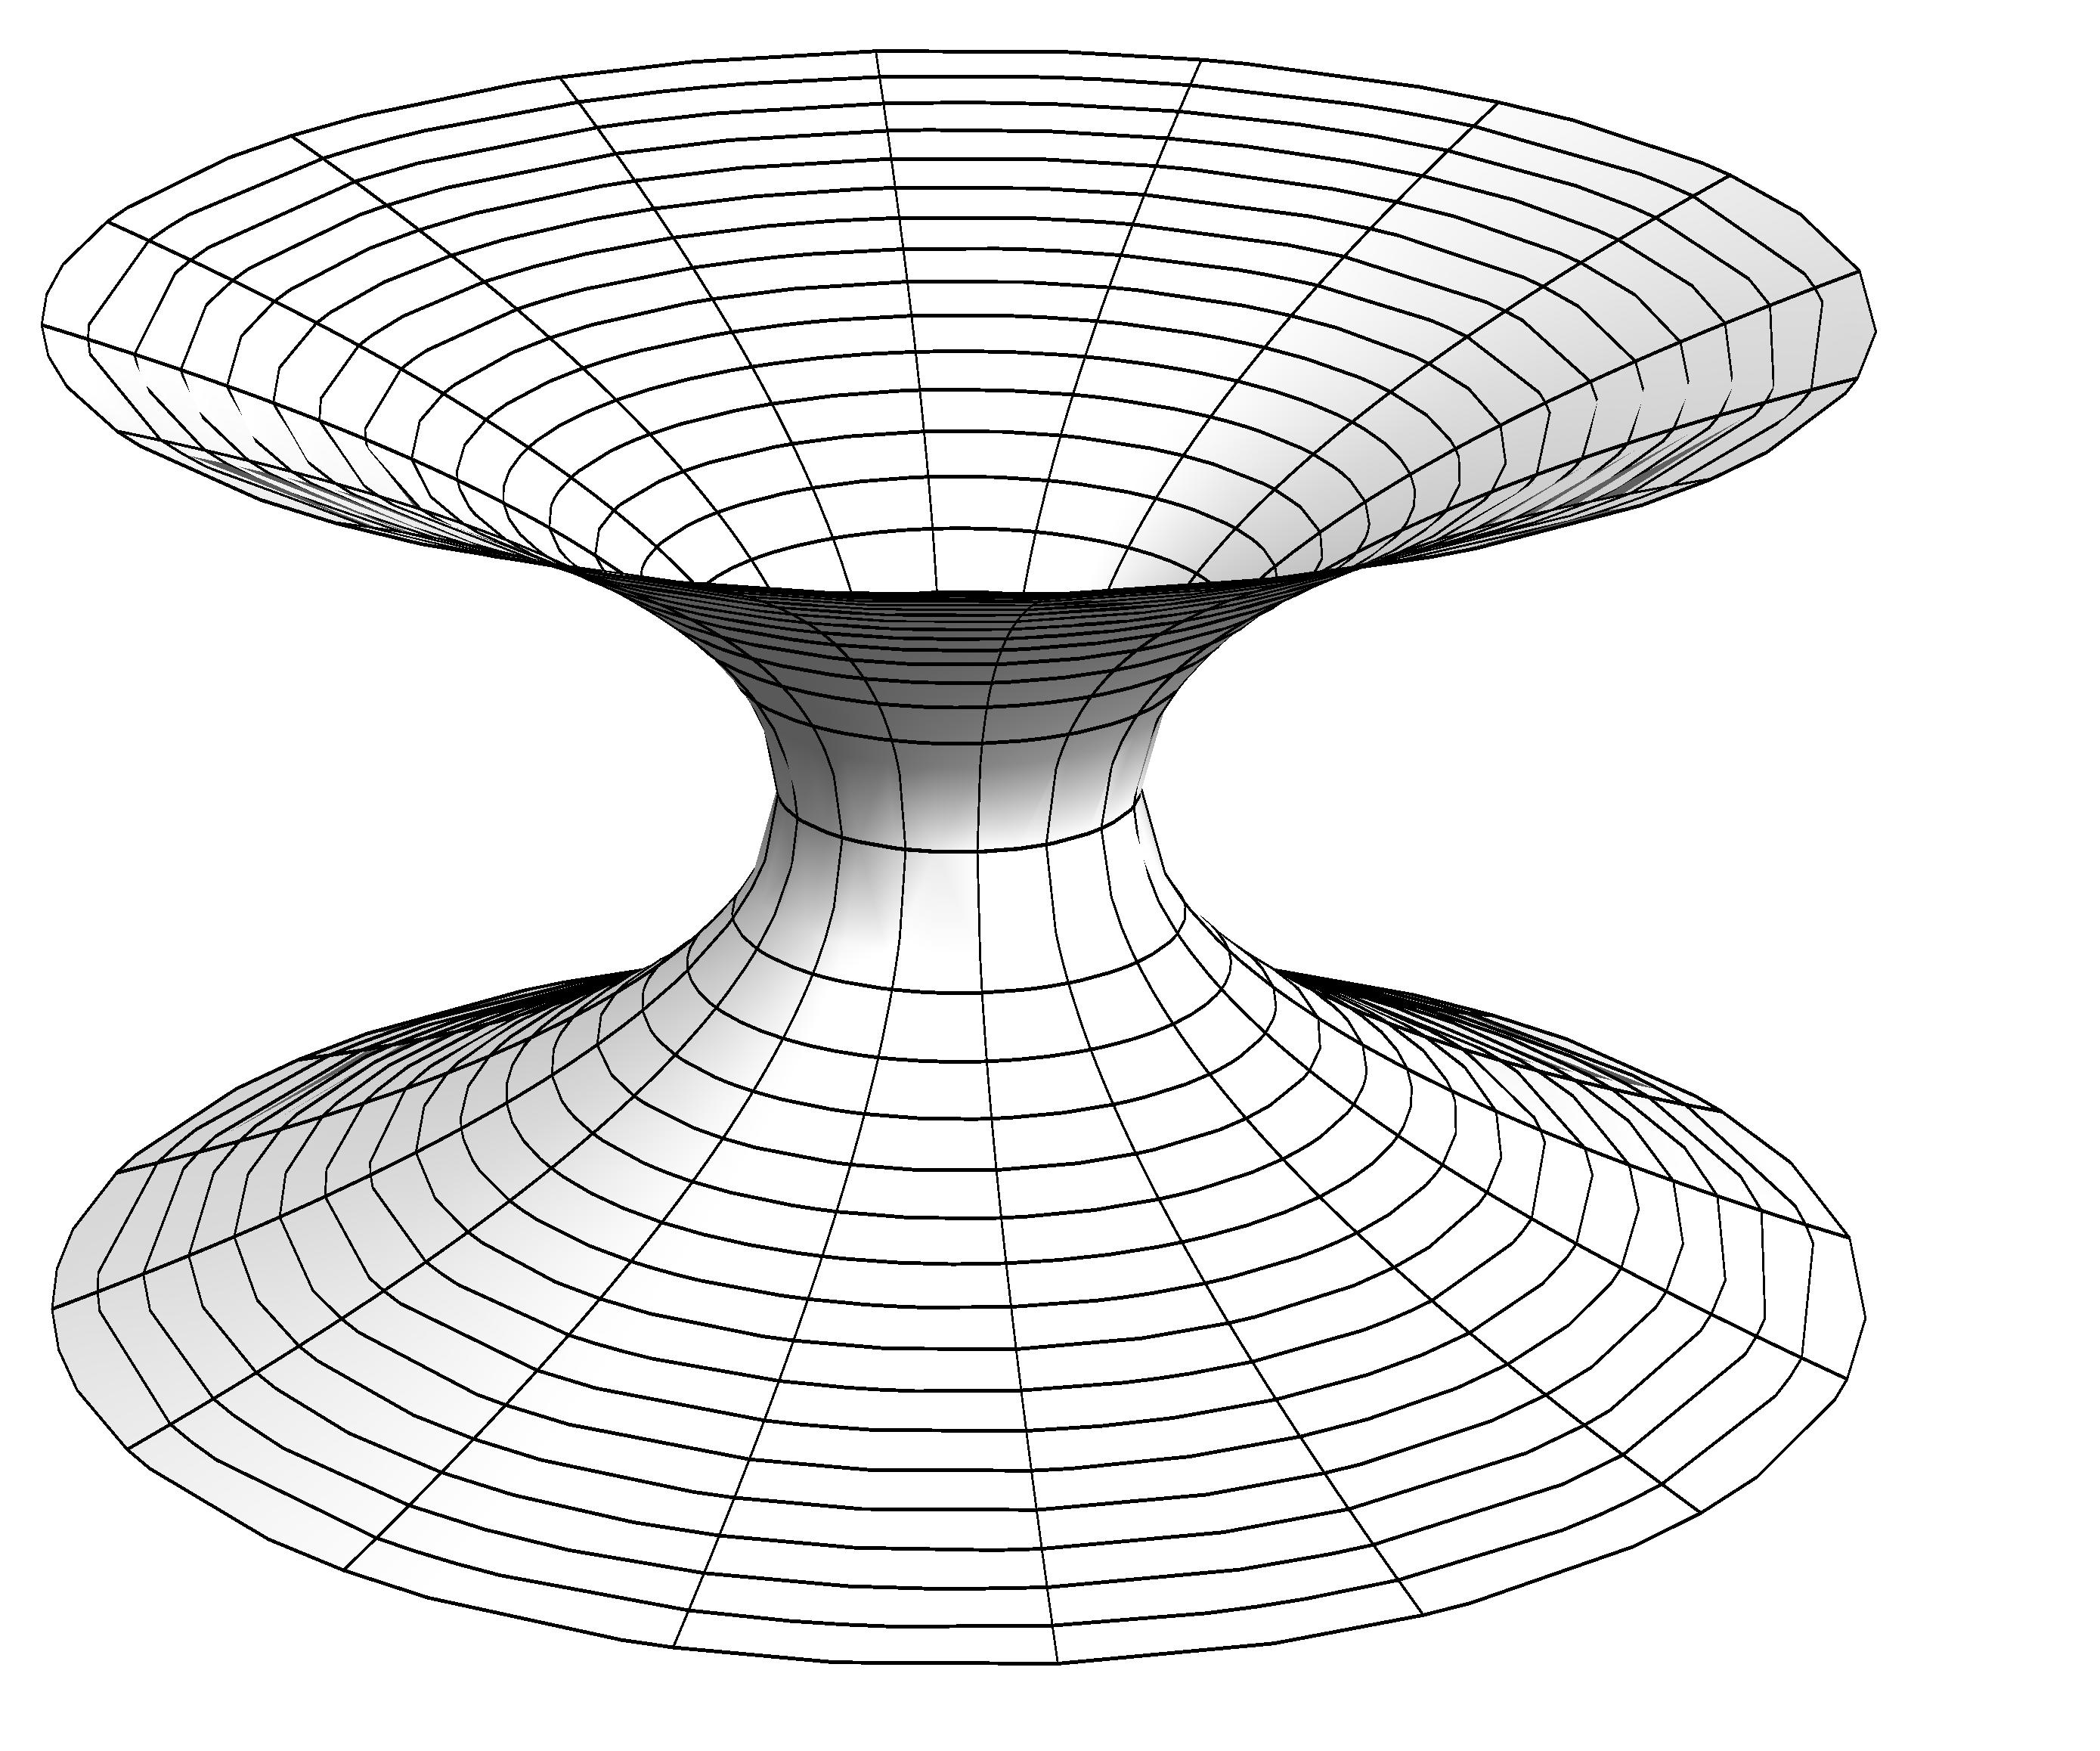
\includegraphics[width=\textwidth]{img/wormhole}
      }{
        Mark Hannam
      }
      \caption{\\Surface with circular symmetry but no coordinate $r = 0$.}
    \end{figure}
  \end{column}

  \begin{column}{0.6\textwidth}
    \begin{itemize}
    \item<+-> ``curvature'' or ``area'' coordinate
      \begin{itemize}
      \item radius of curvature and area
      \end{itemize}
    \item<+-> \emph{not} proper distance from center
    \item<+-> $r =$ const, $t =$ const
      \begin{itemize}
      \item $A = 4 \pi r^2$
      \item $C = 2 \pi r$
      \end{itemize}
    \end{itemize}
  \end{column}
\end{columns}

\blankfootnote{\textcite[p. 257]{Schutz}}

\end{frame}

%%%%

\begin{frame}{Spherically symmetric spacetime}

\begin{block}{General metric}
  \begin{displaymath}
    \dd{s}^2 =
    g_{00} \dd{t}^2 +
    2 g_{0r} \dd{r} \dd{t} +
    g_{rr} \dd{r}^2 +
    r^2 \dd\Omega^2
  \end{displaymath}
\end{block}

\begin{center}
$g_{00}$, $g_{0r}$, and $g_{rr}$ functions of $t$ and $r$
\end{center}

\blankfootnote{\textcite[p. 258]{Schutz}}

\end{frame}

%%%%%%%%

\section{Static spacetimes}


\begin{frame}{Motivation}

\begin{itemize}
\setlength\itemsep{24pt}
\item<+-> leads to simple derivation of Schwarzschild metric
\item<+-> generalizes to spherically symmetric, asymptotically flat Einstein vacuum field equations
\item<+-> Birkhoff's theorem
\end{itemize}

\blankfootnote{\textcite[p. 263]{Schutz} and \textcite[p. 843]{MTW}}


\note{

  \begin{itemize}
  \item Birkhoff's theorem says that the Schwarzschild metric applies to point 2
  \end{itemize}

}

\end{frame}


\begin{frame}{Definition}

A spacetime is static if we can find a time coordinate $t$ for which

\begin{enumerate}[(i)]
\item<+-> the metric independent of $t$

  \begin{displaymath}
    g_{\alpha\beta,t} = 0
  \end{displaymath}

\item<+-> the geometry unchanged by time reversal

  \begin{displaymath}
    t \to -t
  \end{displaymath}

\end{enumerate}

\blankfootnote{\textcite[p. 258]{Schutz}}

\note{

  \begin{itemize}
  \item a spacetime which only satisfies the first condition is \emph{stationary}
    \begin{itemize}
    \item e.g. rotating star
    \end{itemize}
  \end{itemize}

}

\end{frame}

%%%%

\begin{frame}{Time reversal}

\onslide<+->{

\begin{displaymath}
  \vb{\Lambda}: (t, x, y, z) \to (-t, x, y, z)
\end{displaymath}

\begin{displaymath}
  g_{\bar\alpha \bar\beta} =
  \tensor{\Lambda}{^\alpha_{\bar\alpha}}
  \tensor{\Lambda}{^\beta_{\bar\beta}}
  g_{\alpha\beta} =
  g_{\alpha\beta}
\end{displaymath}

}

\begin{columns}[t]
  \begin{column}{0.4\textwidth}
    \begin{block}<+->{Transformation}
      \begin{align*}
          \tensor{\Lambda}{^0_{\bar0}} &=
          \tensor{x}{^0_{,\bar0}} = -\tensor{x}{^0_{,0}} = -1
          \\
          \tensor{\Lambda}{^i_{\bar{j}}} &=
          \tensor{x}{^i_{,\bar{j}}} = \tensor{x}{^i_{,j}} = \tensor{\delta}{^i_j}
          \\
          \tensor{\Lambda}{^0_{\bar{i}}} &=
          \tensor{x}{^0_{,\bar{i}}} = \tensor{x}{^0_{,i}} = 0
        \end{align*}
    \end{block}
  \end{column}

  \begin{column}{0.4\textwidth}
    \begin{block}<+->{Metric}
      \begin{align*}
        g_{\bar0 \bar0} &=
        (\tensor{\Lambda}{^0_{\bar0}})^2 g_{00} =
        g_{00}
        \\
        g_{\bar0 \bar{r}} &=
        \tensor{\Lambda}{^0_{\bar0}} \tensor{\Lambda}{^r_{\bar{r}}} g_{0r} =
        -g_{0r}
        \\
        g_{\bar{r} \bar{r}} &=
        (\tensor{\Lambda}{^r_{\bar{r}}})^2 g_{rr} =
        g_{rr}
      \end{align*}
    \end{block}
  \end{column}
\end{columns}

\blankfootnote{\textcite[p. 258]{Schutz}}


\note{

  \begin{itemize}
  \item $g_{\bar0 \bar{r}} = -g_{0r} = 0$
  \end{itemize}

}

\end{frame}

%%%%

\begin{frame}{The metric}

\begin{block}<+->{Simplified metric}
\begin{displaymath}
  \dd{s}^2 =
  g_{00} \dd{t}^2 +
  g_{rr} \dd{r}^2 +
  r^2 \dd\Omega^2
\end{displaymath}
\end{block}

\begin{block}<+->{Replacement}
\begin{displaymath}
  g_{00} \to -e^{2\Phi},
  \quad
  g_{rr} \to e^{2\Lambda},
  \quad
  \text{provided $g_{00} < 0 < g_{rr}$}
\end{displaymath}
\end{block}

\begin{block}<+->{Static spherically symmetric metric}
\begin{displaymath}
  \dd{s}^2 =
  -e^{2\Phi} \dd{t}^2 +
  e^{2\Lambda} \dd{r}^2 +
  r^2 \dd\Omega^2
\end{displaymath}
\begin{displaymath}
  \lim_{r\to\infty} \Phi(r) = \lim_{r\to\infty} \Lambda(r) = 0
\end{displaymath}
\end{block}

\blankfootnote{\textcite[pp. 258--259]{Schutz}}


\note{

  \begin{itemize}
  \item constraint $g_{00} < 0 < g_{rr}$ holds for stars but not black holes
  \item limits at infinity tell us that spacetime is \emph{asymptotically flat}
  \end{itemize}

}

\end{frame}

%%%%

\begin{frame}{Einstein Tensor}

\begin{block}<+->{General Einstein tensor}
\begin{displaymath}
  G_{\alpha\beta} = R^{\alpha\beta} - \frac{1}{2} g_{\alpha\beta} R
\end{displaymath}
\end{block}

\begin{block}<+->{Einstein tensor components}
\begin{gather*}
  G_{tt} =
  \frac{1}{r^2} e^{2\Phi} \dv{r} [r (1 - e^{-2\Lambda})],
  \\
  G_{rr} =
  -\frac{1}{r^2} e^{2\Lambda} (1 - e^{-2\Lambda}) + \frac{2}{r} \Phi'
  \\
  G_{\theta\theta} =
  r^2 e^{-2\Lambda} [\Phi'' + (\Phi')^2 + \Phi' / r - \Phi' \Lambda' - \Lambda' / r],
  \\
  G_{\phi\phi} =
  \sin^2\theta G_{\theta\theta}
\end{gather*}
\end{block}

\blankfootnote{\textcite[pp. 165, 260]{Schutz}}


\note{

  \begin{itemize}
  \item $x' \equiv \dv*{x}{r}$
  \end{itemize}

}

\end{frame}

%%%%%%%%

\section{Static perfect fluid}


\begin{frame}{Four-velocity}

\begin{block}<+->{Constraints}
\begin{align*}
  U^i &= 0
  \text{ (static)}
  &
  \vec{U} \cdot \vec{U} &= -1
  \text{ (conservation law)}
\end{align*}
\end{block}

\begin{block}<+->{Solving for $U^0$}
\begin{displaymath}
  g_{00} (U^0)^2 = -1 \implies
  U^0 = (-g_{00})^{-1/2} = e^{-\Phi}
\end{displaymath}
\end{block}

\begin{block}<+->{Solving for $U_0$}
\begin{displaymath}
  U_0 = g_{00} U^0 = -e^{\Phi}
\end{displaymath}
\end{block}

\blankfootnote{\textcite[p. 260]{Schutz}}


\note{

  \begin{itemize}
  \item ``conservation law'' is the conservation of four-momentum
  \end{itemize}

  \begin{align*}
    g_{00} U^0 U^0 = -1 \implies
    (U^0)^2 &= (-g_{00})^{-1}
    \\ \implies
    U^0 &= (-g_{00})^{-1/2}
    \\ \implies
    U^0 &= (e^{2\Phi})^{-1/2} = e^{-\Phi}
  \end{align*}

}

\end{frame}

%%

\begin{frame}{Stress--energy tensor}

\begin{block}<+->{$T_{\alpha\beta}$ for perfect fluid}
\begin{displaymath}
  T_{\alpha\beta} = (\rho + p) U_\alpha U_\beta + p g_{\alpha\beta}
\end{displaymath}
\end{block}

\begin{block}<+->{Components of $T_{\alpha\beta}$}
\begin{align*}
  T_{00} &= (\rho + p) e^{2\Phi} + p (-e^{2\Phi}) = \rho e^{2\Phi}
  \\
  T_{\alpha\beta} &= 0 \text{ for $\alpha \neq \beta$;}
  \quad
  T_{ii} = p g_{ii}
  \\
  T_{rr} &= p e^{2\Lambda};
  \quad
  T_{\theta\theta} = p r^2;
  \quad
  T_{\phi\phi} = p r^2 \sin^2\theta = T_{\theta\theta} \sin^2\theta
\end{align*}
\end{block}

\blankfootnote{\textcite[p. 260]{Schutz}}


\note{

  \begin{itemize}
  \item $T_{\alpha\beta} = 0$ because
    \begin{itemize}
    \item the cross terms make $g_{\alpha\beta} = 0$
    \item $T_{0i}$ makes one of the $U$'s $U_i = 0$
    \end{itemize}
  \item likewise, $T_{ii} = p g_{ii}$ because $U_i U_i = 0$
  \end{itemize}

}

\end{frame}

%%%%

\begin{frame}{Equation of state}

\begin{block}{Local thermodynamic equilibrium}
\begin{displaymath}
  p = p(\rho, S) \approx p(\rho)
\end{displaymath}
\end{block}

\begin{itemize}
\item pressure related to energy density and specific entropy
\item we often deal with negligibly small entropies
\end{itemize}

\blankfootnote{\textcite[p. 261]{Schutz}}

\end{frame}

%%%

\begin{frame}{Equations of motion}

\begin{block}<+->{Conservation laws}
\begin{displaymath}
  \tensor{T}{^{\alpha\beta}_{;\beta}} = 0
\end{displaymath}
\end{block}

\begin{itemize}
\item<+-> symmetries make only non-trivial solution $\alpha = r$

\textbf{TODO: prove}
\end{itemize}

\begin{block}<+->{Equation of motion}
\begin{displaymath}
  (\rho + p) \dv{\Phi}{r} = -\dv{\rho}{r}
\end{displaymath}
\end{block}

\blankfootnote{\textcite[pp. 175, 261]{Schutz}}

\end{frame}

%%%%

\begin{frame}{Equation of motion (continued)}

\textbf{TODO}

Show 10.31

\end{frame}

%%%%%%%%

\section{Exterior Geometry}


\begin{frame}{Schwarzschild metric}

\textbf{TODO}

\end{frame}

%%%%

\begin{frame}{Birkhoff's Theorem}

\onslide<+-> {

Let the geometry of a given region of spacetime:

}

\begin{enumerate}
\item<+-> be spherically symmetric
\item<+-> be a solution to the Einstein field equations in vacuum.
\end{enumerate}

\onslide<+->{

Then that geometry is necessarily a piece of the Schwarzschild geometry.

}

\vspace{0.5in}

\onslide<+->{

(Proof given in \textcite[pp. 843--844]{MTW})

}

\blankfootnote{\textcite{1923rmp..book.....B}}

\end{frame}




\section{References}

\begin{frame}[allowframebreaks]

\nocite{*}
\printbibliography[heading=subbibliography]

\end{frame}

\end{document}
